\documentclass[a5paper,8pt,twoside]{extarticle}
\usepackage[utf8]{inputenc}
\usepackage[IL2]{fontenc}
\usepackage{geometry}
\geometry{outer=2cm,top=2cm,bottom=2cm}
\usepackage{tikz}
\usepackage{enumitem}
\graphicspath{ {img/} }
\usepackage[english,main=czech]{babel}
\usepackage{blindtext}
\usepackage{pifont,mdframed}
\usepackage{fourier}
\usepackage{icomma}
\usepackage{tabularx}
\usepackage[unicode,hidelinks]{hyperref}
\usepackage{multicol}
\usepackage[compact]{titlesec}
\newcommand{\email}[1]{\texttt{\href{mailto:#1}{#1}}}
\newenvironment{warningBox}
  {\par\begin{mdframed}[linewidth=1pt,linecolor=black]%
    \begin{list}{}{\leftmargin=1cm
                   \labelwidth=\leftmargin}\item[\Large\warning]}
  {\end{list}\end{mdframed}\par}
  
  \newenvironment{infoBox}
  {\par\begin{mdframed}[linewidth=1pt,linecolor=black]%
    \begin{list}{}{\leftmargin=1cm
                   \labelwidth=\leftmargin}\item[\Large\lefthand]}
  {\end{list}\end{mdframed}\par}

  \newenvironment{prohibitBox}
  {\par\begin{mdframed}[linewidth=1pt,linecolor=black]%
    \begin{list}{}{\leftmargin=1cm
                   \labelwidth=\leftmargin}\item[\Large\noway]}
  {\end{list}\end{mdframed}\par}

   \newenvironment{function_reference}[1]
   {\par
    \begin{list}{}{\leftmargin=1cm
                   \labelwidth=\leftmargin}\item[{\raisebox{-0.5\baselineskip}{\includegraphics[height=1.5\baselineskip]{#1}}}]}
  {\end{list}\par}

  \newenvironment{function_reference_bodge_trig}[1]
   {\par
    \begin{list}{}{\leftmargin=1cm
                   \labelwidth=\leftmargin}\item[{\raisebox{-3.5\baselineskip}{\includegraphics[height=4.5\baselineskip]{#1}}}]}
  {\end{list}\par}

  \newcommand*\joinBox{\vspace{-0.9em}}

  \newenvironment{law}{
    \fontsize{3pt}{3.6pt}
    \selectfont
  }{}

  \newcommand*\lawHead{\fontsize{3.5pt}{4.2pt}}


%%%%%%%%%%%%%%%%%%%%%%%%%%%%%%%%%%%%%%%%%%%%%%%%%%%%%%%%%%%%%%%%%%%%%%
% LaTeX Overlay Generator - Annotated Figures v0.0.1
% Created with http://ff.cx/latex-overlay-generator/
% If this generator saves you time, consider donating 5,- EUR! :-)
%%%%%%%%%%%%%%%%%%%%%%%%%%%%%%%%%%%%%%%%%%%%%%%%%%%%%%%%%%%%%%%%%%%%%%
%\annotatedFigureBoxCustom{bottom-left}{top-right}{label}{label-position}{box-color}{label-color}{border-color}{text-color}
\newcommand*\annotatedFigureBoxCustom[8]{\draw[#5,thick,rounded corners] (#1) rectangle (#2);\node at (#4) [fill=#6,thick,shape=circle,draw=#7,inner sep=2pt,font=\sffamily,text=#8] {\textbf{#3}};}
%\annotatedFigureBox{bottom-left}{top-right}{label}{label-position}
\newcommand*\annotatedFigureBox[4]{\annotatedFigureBoxCustom{#1}{#2}{#3}{#4}{red}{white}{black}{black}}
\newcommand*\annotatedFigureText[4]{\node[draw=none, anchor=south west, text=#2, inner sep=0, text width=#3\linewidth,font=\sffamily] at (#1){#4};}
\newenvironment {annotatedFigure}[1]{\begin{tikzpicture}
\node[anchor=south west,inner sep=0] (image) at (0,0) { #1};\begin{scope}[x={(image.south east)},y={(image.north west)}]}{\end{scope}\end{tikzpicture}}
%%%%%%%%%%%%%%%%%%%%%%%%%%%%%%%%%%%%%%%%%%%%%%%%%%%%%%%%%%%%%%%%%%%%%%

\newcommand*\nref[1]{\textbf{(\ref{#1}, str. \pageref{#1})}}
\newcommand*\fref[2]{\textbf{(obr. \ref{#1}#2, str. \pageref{#1})}}
\newcommand*\cleartoleftpage{%
  \clearpage
  \ifodd\value{page}\hbox{}\newpage\fi
}
\title{CalcIVSulator\\Uživatelský manuál}
\usepackage{}
\author{Lidé u výtahu}
\date{\today}
\begin{document}
    \renewcommand\thesubsubsection{\Alph{subsubsection}}
    \setlength{\parindent}{0em}
    \setlength{\parskip}{1em}
    \begin{titlepage}
        \newgeometry{top=2cm,bottom=2cm,left=2cm,right=2cm}
        \begin{center}
            {\LARGE \textsc{Lidé u výtahu}}

            \vspace{\stretch{0.382}}
            {\large Uživatelský manuál}
            
            {\Huge CalcIVSulator}\\
            \vspace{1.5mm}
            {\huge Pokročilý výpočetní software}\\
            \vspace{\stretch{0.618}}
        \end{center}
        {\large Duben 2020} \hfill {\large Verze 1.0}
    \end{titlepage}
    
    %The following page is the LEFT INSIDE COVER; do not remove this page; keep it blank if need be!
    \thispagestyle{empty}
    \begin{infoBox}
            Copyright \textcopyright{} 2020 Viktor Rucký.

            \foreignlanguage{english}{Permission is granted to copy, distribute and/or modify this document
            under the terms of the GNU Free Documentation License, Version 1.3
            or any later version published by the Free Software Foundation;
            with no Invariant Sections, no Front-Cover Texts, and no Back-Cover Texts.
            A copy of the license is included in the section entitled "GNU
            Free Documentation License".}
    \end{infoBox}
    \joinBox
    \begin{warningBox}
        Skupina Lidé u výtahu se snaží, aby kalkuačka byla pouze co nejpřesnější. Přičemž nemůže garantovat 100\% přesnost a nulovu chybovst výpočtů.

        Používáním kalkulačky souhlasíte, že skupina Lidé u výtahu není zodpovědná za žádnou újmu, materiální či jiného druhu, způsobenou používaní tohoto softwaru.
    \end{warningBox}
    \joinBox
    \begin{warningBox}
        Skupina Lidé u výtahu opovrhuje využívaní tohoto softwaru v akademických kontextech, kde je využívaní kalkulaček zakázáno.

        Skupina Lidé u výtahu nezodpovídá za stanutí před displinární komisí, špatnou známkou či vyloučením plynoucí z používaní tohoto softwaru v nepovelných kontextech.
    \end{warningBox}
    
    \newpage
    \setcounter{page}{1}
    \tableofcontents
    
    \newpage

    \section*{Vítejte}
    Gratulujeme k pořízení kalkulačního software od skupiny Lidé~u~výtahu. Jsem si jistí, že náš software Vás nezklame. Ba naopak. Náš software prošel sofistikovaným plánování a vývojem, typické pro inženýry vycházející z nejprestižnějších univerzitních institucí, a zaručejeme Vám stoprocentní spokojenost.

    Potřeba počítat je stará, jako písmo\,--\,mnohé nejstarší dochovalé písemnosti mluví o počtech, o daních. Čísla jsou prostě spjatá s lidskou civilizací. Již staří Egypťané vynalezli abakus\,--\,kuličkové počítadlo\,--\,zařízení pro zjednodušení počtů. A jak se velikost lidských společností zvětšovala, tak i její potřeba pro rychlé a efektivní výpočty. Historie moderních početních zařízení počala roku 1642 vynálezem mechanické kalkulačky Wilhelmem Schickerdem. A jak tato historie postupovala, přes logaritmická pravítka, elektromechanické kalkulátory, počítače založené na relé i tranzistorech, tak se dostala do rukou i nám. S radostí Vám představuje nejnovější eveluci ve světe výpočtů.

    A tímto evoluce nekončí, jak vývoj dnešních technoligií postupuje raketově dopředu, tak postupujeme my: náš software je neustále aktualizován a vyvíjen; jsme odhodlaní přidávat funkce a zůstat na vrcholu výpočetního software.
    
    ---Viktor Rucký, zakladatel skupiny Lidé u výtahu
    \newpage
    \section{Instalace}
    TODO
    \section{Spuštění}
    TODO
    \cleartoleftpage
    \section{Užívání}
    \subsection{Uživatelské rozhraní\,--\,obecné}
    \begin{figure}[h]
        \begin{center}
            \begin{annotatedFigure}
                {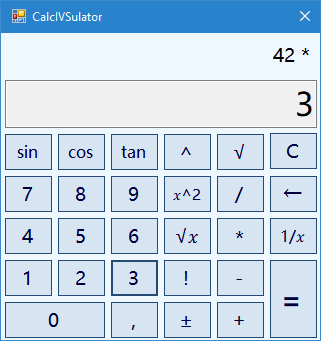
\includegraphics[width=0.75\linewidth]{calculator.PNG}}
                \annotatedFigureBox{0.01,0.0077}{0.9919,0.6176}{A}{0.01,0.31265}%bl
                \annotatedFigureBox{0.01,0.6176}{0.9919,0.7746}{B}{0.01,0.6961}%bl
                \annotatedFigureBox{0.01,0.7746}{0.9919,0.8875}{C}{0.01,0.83105}%bl
                \annotatedFigureBox{0.9,0.9}{1,1}{D}{0.885,0.95}%bl
            \end{annotatedFigure}
        \end{center}
    \caption{Hlavní sekce uživatelského rozhraní}
    \label{fig:UI_main}
    \end{figure}
    Uživatelské rozhraní je tvořeno čtyřmi častmi:

    \subsubsection{Klávesnice}
    Pomocí klávesnice lze zadat data do kalkulačky. Princip operace je vysvětlen v sekci \uv{obecné používaní} \nref{sec:general_use}. Funkce jednotlivých tlačítek je vysvětlena v sekci \uv{uživatelské rohraní\,--\,klávesnice} \nref{sec:UI_keyboard}.

    \subsubsection{Výsledkový a zadávací displej}
    Zde se zobrazí výsledek Vaši operace nebo právě zadaný operand.

    \subsubsection{Displej s předchozí operací}
    Zde se zobrazí předchozí operand a operace, která je prováděna.

    \subsubsection{Ukončovací křížek}
    Pomocí křížku lze ukončit aplikaci.

    \subsection{Uživatelské rohraní\,--\,klávesnice}
    \label{sec:UI_keyboard}
    \begin{figure}[h]
        \begin{center}
        \begin{annotatedFigure}
            {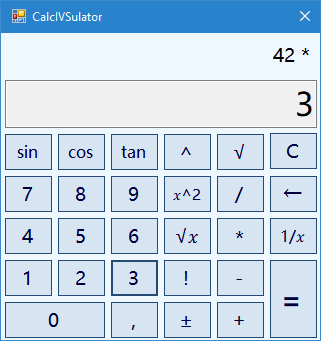
\includegraphics[width=0.75\linewidth]{calculator.PNG}}
            \draw[red, thick, rounded corners] (0.01,0.005) -- (0.335,0.005) -- (0.335, 0.123125) -- (0.5, 0.123125) -- (0.5,0.4925) -- (0.01,0.4925) -- cycle;
            \node at (0.01,0.24875) [fill=white,thick,shape=circle,draw=black,inner sep=2pt,font=\sffamily,text=black] {\textbf{A}};
            \annotatedFigureBox{0.335,0.005}{0.5, 0.123125}{B}{0.4175,-0.01}%bl
            \annotatedFigureBox{0.5,0.005}{0.665, 0.123125}{C}{0.5825,-0.01}%bl
            \annotatedFigureBox{0.83,0.37}{0.9919, 0.4925}{D}{1,0.43125}%bl
            \annotatedFigureBox{0.83,0.4925}{0.9919, 0.615}{E}{1,0.55375}%bl
            \annotatedFigureBox{0.83,0.005}{0.9919, 0.2475}{G}{1,0.12625}%bl
            \draw[green, thick, rounded corners] (0.01,0.4925) -- (0.01,0.615) -- (0.83,0.615) -- (0.83, 0.37) -- (0.9919, 0.37) -- (0.9919,0.2475) -- (0.83,0.2475) -- (0.83,0.005) -- (0.665,0.005) -- (0.665, 0.123125) -- (0.5,0.123125) -- (0.5,0.4925) -- cycle;
            \node at (0.01,0.55375) [fill=white,thick,shape=circle,draw=black,inner sep=2pt,font=\sffamily,text=black] {\textbf{F}};
        \end{annotatedFigure}
      \end{center}
        \caption{Rozdělení klávesnice}
        \label{fig:UI_keyboard}
    \end{figure}
    Klávesnici kalkulačky lze rozdělit do několika funkčních celků.

    \subsubsection{Numerické klávesy}
    Používají se pro zadávání čísel operandů, spolu s klávesami \uv{desetinná čárka} \textbf{(B)} a \uv{změ\-na znaménka} \textbf{(C)}. Viz. sekce \uv{zadávání čísel} \nref{sec:entering_numbers}.

    \subsubsection{Desetinná čárka}
    Pro zadávní desetinné čarky při vkládání čísel. Viz. sekce \uv{zadávání čísel} \nref{sec:entering_numbers}.

    \subsubsection{Změna znaménka}
    Pro změnu znaménka zadaného čísla. Viz. sekce \uv{zadávání čísel} \nref{sec:entering_numbers}.

    \subsubsection{Smazání číslice}
    Smaže poslední číslici (číslici nejnižšího řádu) ve \uv{výsledkovém a zadávacím displeji} \fref{fig:UI_main}{.B}. Viz. sekce \uv{zadávání čísel} \nref{sec:entering_numbers}.

    \subsubsection{Smazat vše}
    Smaže obsah kalkulačky, včetně přechozího čísla a operace. Viz. sekce \uv{obecné používaní} \nref{sec:general_use}.

    \subsubsection{Tlačítka funkcí a operací}
    Tyto tlačítka slouží pro výběr provedené funkce či operace nad zadanými čísly. Viz. sekce \uv{funkce kalkulačky} \nref{sec:function_reference}.

    \subsubsection{Rovná se / potrvrzení}
    Tímto se potvrdí zadané číslo a provede se zadaná binární operace. Viz. sekce \uv{obecné používaní} \nref{sec:general_use}.

    \subsection{Obecné používání}
    \label{sec:general_use}
    Proces pro většinu operací s kalkulačkou je následující. Doporučujeme také přečíst sekci \uv{zadávaní čísel} \nref{sec:entering_numbers}. Jednotlivé funkce a operace kalkulačky jsou popsány v sekci \uv{funkce kalkulačky} \nref{sec:function_reference}.
    \begin{enumerate}
        \item Zadejte číslo prvního operandu pomocí \uv{numerických kláves}, a pokud je třeba, kláves \uv{desetinné čárky} anebo \uv{změny znaménka} \fref{fig:UI_keyboard}{.A/B/C}.
        \item Vyberte požadovanou operaci pomocí \uv{klávesy funkce nebo operace} \fref{fig:UI_keyboard}{.F}.
        \item Pokud je operace unární, zobrazí se výsledek (nebo chybové hlášení) na \uv{vý\-sled\-ko\-vém a zadávacím displeji} \fref{fig:UI_main}{.B}, jinak se zadáný operand a symbol operace zobrazí na \uv{displeji s předchozí operací} \fref{fig:UI_main}{.C}.
        \item Obdobně jako první operand, zadejte druhý operand.
        \item Potvrďte druhý operand pomocí klávesy \uv{rovná se / potrvrzení} \fref{fig:UI_keyboard}{.G}.
        \item Na \uv{výsledkovém a zadávacím displeji} se zobrazí výsledek nebo chybové hlášení; o chybových hlášeních Vás informujeme v sekci \uv{chybová hlášení} \nref{sec:errors}.
    \end{enumerate}
    Pokud jste udělali chybu v zadání prvního operandu nebo ve výběru operace, stisknětě klávesu \uv{smazat vše} \fref{fig:UI_keyboard}{.E}.
    \begin{infoBox}
        Kalkulačka používá infixní notaci!
    \end{infoBox}
    \joinBox
    \begin{infoBox}
        Kalkulačka neuplatňuje prioritu operátorů!
    \end{infoBox}
    \joinBox
    \begin{warningBox}
        Kalkulačka se snaží býti velice přesná a má nízkou chybu při výpočtech. Opakované využítí výsledku v operacích způsobuje kumulování chyby, což může snížit přesnost.
    \end{warningBox}
    \subsection{Zadávání čísel}
    \label{sec:entering_numbers}
    Kalkulačka dokáže pracovat s kladnímy celými čísly ale i čísly desetinnímy a zápornými.

    Aktualné zadávané číslo se zobrazí ve \uv{výsledkovém a zadávacím displeji} \fref{fig:UI_main}{.B}.

    Pomocí \uv{numerických kláves} \fref{fig:UI_keyboard}{.A} se zadávají jednotlivé číslice. Vložená číslice se zobrazí na místě jednotek a předchozí číslo se posune o řád doleva, aby vytvořilo místo pro novou číslici (mimo situaci po stisknutí klávesy \uv{desetinná čárka}).

    Pomocí klávesy \uv{desetinná čárka} \fref{fig:UI_keyboard}{.B} se zobrazí desetinná čárka za číslicí řádu jednotek. Nyní se po stiknutí \uv{numerických kláves} nová číslice zobrazí na pravém konci čísla (tj. místě s řádem o jedna menší, než řád již zadané číslice s nejnižším řádem).

    \begin{prohibitBox}
        Opětovné stisknutí klávesy \uv{desetinná čárka} \textbf{nezpůsobí} změnu umístění desetinné čarky! Pomocí klávesy \uv{smazání číslice} je třeba desetinnou čá\-rku nejprve smazat!
    \end{prohibitBox}

    Pokud chcete zadat číslo záporné, použijte klávesu \uv{změna znaménka} \fref{fig:UI_keyboard}{.C}. Opětovné stisknutí klávesy změní zadané číslo zpět na číslo kladné.

    \begin{prohibitBox}
        Nesnažte se zadat záporné číslo pomocí klávesy \uv{odčítání}! Je nutné použít klávesu \uv{změna znaménka}!
    \end{prohibitBox}

    Pokud provedete chybu při zadávání čísla, lze smazat poslední číslici pomocí klávesy \\\uv{sma\-zá\-ní čí\-sli\-ce} \fref{fig:UI_keyboard}{.D}; klávesu lze použít opakovaně. Pokud chcete smazat celé číslo, můžete využít klávesu \uv{smazat vše} \fref{fig:UI_keyboard}{.E}.

    \begin{warningBox}
        Použítí klávesy \uv{smazat vše} také smaže předchozí operand a vybranou operaci.
    \end{warningBox}

    \renewcommand\thesubsubsection{\thesubsection.\arabic{subsubsection}}
    \subsection{Jednotlivé funkce kalkulačky}
    \label{sec:function_reference}
    V této sekci jsou popsány funkce všech \uv{kláves funckí a operací} \fref{fig:UI_keyboard}{.F}.

    \subsubsection{Sčítaní}
    \label{sec:addition}
    \begin{function_reference}{btn_plus}
        Sečte operandy.
    \end{function_reference}
    
    \subsubsection{Odčítaní}
    \label{sec:subtraction}
    \begin{function_reference}{btn_minus}
        Odečte druhý operand od prvního.
    \end{function_reference}

    \subsubsection{Násobení}
    \label{sec:multiply}
    \begin{function_reference}{btn_multiply}
        Vynásobí operandy.
    \end{function_reference}

    \subsubsection{Dělení}
    \label{sec:division}
    \begin{function_reference}{btn_divide}
        Vydělí první operand druhým.
        \begin{infoBox}
            Pro rychlý výpočet obráceného čísla lze využít funkci \uv{obrácené číslo} \nref{sec:inverse}.
        \end{infoBox}
        \joinBox
        \begin{prohibitBox}
            Dělení nulou není definované a způsobí chybové hlášení!
        \end{prohibitBox}
    \end{function_reference}

    \subsubsection{Druhá mocnina}
    \label{sec:square}
    \begin{function_reference}{btn_square}
        Umocní operandu na druhou.
        \begin{infoBox}
            Pro obecnou mocninu použijte funkci \uv{obecná mocnina} \nref{sec:power}.
        \end{infoBox}
    \end{function_reference}

    \subsubsection{(Obecná) mocnina}
    \label{sec:power}
    \begin{function_reference}{btn_power}
        Umocní první operand na druhý. Jsou podporováný i záporné mocniny.
        \begin{infoBox}
            Pro rychlý výpočet druhé mocniny lze využít funkci \uv{druhá mocnina} \nref{sec:square}.
        \end{infoBox}
        \joinBox
        \begin{prohibitBox}
            Druhý operand musí být celé číslo! Jinak se zobrazí chybové hlášení!
        \end{prohibitBox}
        \joinBox
        \begin{prohibitBox}
            Operace $0^0$ není definována a způsobí chybové hlášení!
        \end{prohibitBox}
    \end{function_reference}

    \subsubsection{(Druhá) odmocnina}
    \label{sec:sqrt}
    \begin{function_reference}{btn_sqrt}
        Vypočítá druhou odmocninu zadaného čísla.
        \begin{infoBox}
            Pro obecnou odmocninu využijte funkci \uv{obecná odmocnina}\\ \nref{sec:root}.
        \end{infoBox}
        \joinBox{}
        \begin{prohibitBox}
            Kalkulačka nepodporuje komplexní odmocninu!\\
            Odmocnina záporných čísel není definována a způsobí chybové hlášení!
        \end{prohibitBox}
    \end{function_reference}

    \subsubsection{Obecná odmocnina}
    \label{sec:root}
    \begin{function_reference}{btn_root}
        Odmocní první operand řádem druhého operandu.
        \begin{infoBox}
            Pro rychlý výpočet druhé odmocniny lze využít funkci \uv{druhá odmocnina} \nref{sec:sqrt}.
        \end{infoBox}
        \joinBox
        \begin{prohibitBox}
            Kalkulačka nepodporuje komplexní odmocninu!\\
            Odmocnina záporných čísel se sudým odmocněncem není definována a způsobí chybové hlášení!
        \end{prohibitBox}
        \joinBox
        \begin{prohibitBox}
            Odmocnění nuly se záporným řádem není definována a způsobí chybové hlášení!
        \end{prohibitBox}
        \joinBox
        \begin{prohibitBox}
            Odmocnina nultého řádu není definována a způsobí chybové hlášení!
        \end{prohibitBox}
    \end{function_reference}

    \subsubsection{Faktoriál}
    \label{sec:factorial}
    \begin{function_reference}{btn_factorial}
        Vypočítá faktoriál operandu.
        \begin{infoBox}
            Kalkulačka dokáže spočítat faktoriálý čísel do hodnoty 170.
        \end{infoBox}
        \joinBox
        \begin{prohibitBox}
            Faktoriál záporných a desetinných čísel není definovaný a způsobí chybové hlašení!
        \end{prohibitBox}
    \end{function_reference}

    \subsubsection{Goniometrické funkce}
    \label{sec:trig}
    \begin{function_reference_bodge_trig}{btn_trig}
        Vypočítá vybranou goniometrickou funkci\,--\,sinus, kosinus, nebo tangens. Úhel

        \vspace{-4.5em} je zadaný v radiánech.
        \begin{warningBox}
            Je třeba zadat argument goniometrických funkcí v radiánech.
        \end{warningBox}
        \joinBox
        \begin{prohibitBox}
            Tangens $(2k+1)\pi, k \in \mathbb{Z} $ není definovaný a způsobí chybové hlášení.
        \end{prohibitBox}
    \end{function_reference_bodge_trig}

    \subsubsection{Obrácené číslo}
    \label{sec:inverse}
    \begin{function_reference}{btn_inverse}
        Vypočíta obrácené číslo operandu.
        \begin{infoBox}
            Tato operance je ekvivalentní k operaci $1 / X$ \nref{sec:division}.
        \end{infoBox}
        \joinBox
        \begin{prohibitBox}
            Obrácené číslo nuly není definované a způsobí chybové hlášení.
        \end{prohibitBox}
    \end{function_reference}

    \subsection{Chybová hlášení}
    \label{sec:errors}

    Při operaci kalkulačky mohou nastat chybová hlášení.

    \subsubsection{No input given}
    Nezadal jste žádný operand.

    \subsubsection{Overflow chyba}
    Požadovaná operace vrátilo číslo mimo kalkulační rozsah kalkulátoru.

    \subsubsection{Dělení nulou}
    Dělíte nulou nebo se pokušíte provést operaci, která interně se o dělení nulou snaží.

    Podívejte se na nedefinované vstupní hodnoty funkce, kterou se snažíte použít v sekci \uv{jednotlivé funkce kalkualčky} \nref{sec:function_reference}.

    \subsubsection{Nepovolená operace}
    Snažíte se provést operaci se vstupem, který není platný.
    
    Podívejte se na nedefinované vstupní hodnoty funkce, kterou se snažíte použít v sekci \uv{jednotlivé funkce kalkualčky} \nref{sec:function_reference}.

    \subsubsection{Wrong input}
    Zadaný vstup není platný.

    Podívejte se na nedefinované vstupní hodnoty funkce, kterou se snažíte použít v sekci \uv{jednotlivé funkce kalkualčky} \nref{sec:function_reference}.    

    \subsection{Zobrazení nápovědy}
    Stisknutím klávesy \uv{F1} v otevřeném programu CalcIVSulator se zobrazí elektronická verze této uživatelské příručky; verze tištěné a elektronické příručky se mohou lišit.

    \begin{infoBox}
        Pro zobrazení uživatelské příručky je třeba mít ve Vašem počítači nainstalovaný prohlížeč souborů PDF (Portable Document Format). Prohlížeč souborů PDF můžete například zdarma stáhnout z této adresy \url{https://get.adobe.com/cz/reader/}.
    \end{infoBox}

    \subsection{Zobrazení informací o autorech a sestavení programu}
    Stisknutím klávesy \uv{F2} v otevřeném programu CalcIVSulator se zobrazí informace o programu, jeho autorech a verzi.

    \section{Technické informace}

    \begin{table}[h]
    \begin{tabularx}{\textwidth}{|X|X|}
    \hline
    Počet číslic využívaných při vnitřních výpočtech & 15 \\ \hline
    Přesnost & 10 desetinných míst (chyba se kumuluje při opakovaných operací s výsledkem) \\ \hline
    Maximální hodnota využívána kalkulačkou interně& $1,7976931348623157 \cdot 10^{308}$ \\ \hline
    Minimální hodnota využívána kalkulačkou interně & $-1,7976931348623157 \cdot 10^{308}$ \\ \hline
    Maximální vstupní hodnota& $9999999999999999999$ \\ \hline
    Minimální vstupní hodnota& $-9999999999999999999$ \\ \hline
    Nejmenší vstupní hodnota& $0,000000000000000001$ \\ \hline
    \end{tabularx}
    \end{table}

    \section{Autoři}

    Program CalcIVSulator je autorským dílem skupiny Lidé u výtáhu, která je tvořena těmito lidmi:

    \begin{itemize}
        \item Ondřej Sloup (\email{xsloup02@stud.fit.vutr.cz})
        \item Viktor Rucký (\email{xrucky01@stud.fit.vutr.cz})
        \item Vojtěch Vlach (\email{xvlach22@stud.fit.vutr.cz})
    \end{itemize}

    \begin{infoBox}
        Viktor Rucký sbírá pohlednice. Pokud chcete, napište Viktorovi o poštovní adresu e-mailem a pošlete mu pohlednici!
    \end{infoBox}

    \begin{tabularx}{\textwidth}{X X}
        \raisebox{-5em}{
\includegraphics[scale=0.25]{logo_fit.pdf}} & Tento software byl vyvinut jako projekt předmětu IVS studenty Fakulty informačních technoligií Vysokéhu učení technického v Brně.
    \end{tabularx}
    
    \section{Historie}
    \begin{tabularx}{\textwidth}{|l|X|l|}
        \hline
        Verze&Poznámky k verzi&Autoři změn \\ \hline
        1.0&První vydání příručky&Viktor Rucký (\email{xrucky01@stud.fit.vutr.cz}) \\ \hline
    \end{tabularx}

    \section{Licence a právní náležitosti}
    
    \subsection{Licence k programu}
    Tato sekce se váže k softwaru, nikoliv k dokumentaci.
    
    \begin{otherlanguage}{english}
    CalcIVSulator (Simple calculator with GUI and mathematical library)\\
    Copyright \textcopyright{} 2020 Viktor Rucký, Ondřej Sloup, Vojtěch Vlach

    CalcIVSulator is free software: you can redistribute it and/or modify
    it under the terms of the GNU General Public License as published by
    the Free Software Foundation, either version 3 of the License, or
    (at your option) any later version.

    CalcIVSulator is distributed in the hope that it will be useful,
    but WITHOUT ANY WARRANTY; without even the implied warranty of
    MERCHANTABILITY or FITNESS FOR A PARTICULAR PURPOSE.  See the
    GNU General Public License for more details.

    You should have received a copy of the GNU General Public License
    along with CalcIVSulator.  If not, see \url{https://www.gnu.org/licenses/}.
    \end{otherlanguage}

    \subsection{GNU Free Documentation License}
    Tato sekce se váže k této uživatelské příručce.

    \setlength{\parindent}{1em}
\setlength{\parskip}{0em}
\begin{multicols}{2}
\begin{otherlanguage}{english}
\begin{law}
\centerline{
   Version 1.3, 3 November 2008
}

\centerline{Copyright \copyright{} 2000, 2001, 2002, 2007, 2008  Free Software Foundation, Inc.}

\smallskip

    \centerline{<https://fsf.org/>}

\smallskip

\centerline{Everyone is permitted to copy and distribute verbatim copies
of this license document, but changing it is not allowed.}

\centerline{
{\lawHead\bf Preamble}
}

The purpose of this License is to make a manual, textbook, or other
functional and useful document ``free'' in the sense of freedom: to
assure everyone the effective freedom to copy and redistribute it,
with or without modifying it, either commercially or noncommercially.
Secondarily, this License preserves for the author and publisher a way
to get credit for their work, while not being considered responsible
for modifications made by others.

This License is a kind of ``copyleft'', which means that derivative
works of the document must themselves be free in the same sense.  It
complements the GNU General Public License, which is a copyleft
license designed for free software.

We have designed this License in order to use it for manuals for free
software, because free software needs free documentation: a free
program should come with manuals providing the same freedoms that the
software does.  But this License is not limited to software manuals;
it can be used for any textual work, regardless of subject matter or
whether it is published as a printed book.  We recommend this License
principally for works whose purpose is instruction or reference.


\centerline{
{\lawHead\bf 1. APPLICABILITY AND DEFINITIONS\par}
}

This License applies to any manual or other work, in any medium, that
contains a notice placed by the copyright holder saying it can be
distributed under the terms of this License.  Such a notice grants a
world-wide, royalty-free license, unlimited in duration, to use that
work under the conditions stated herein.  The ``\textbf{Document}'', below,
refers to any such manual or work.  Any member of the public is a
licensee, and is addressed as ``\textbf{you}''.  You accept the license if you
copy, modify or distribute the work in a way requiring permission
under copyright law.

A ``\textbf{Modified Version}'' of the Document means any work containing the
Document or a portion of it, either copied verbatim, or with
modifications and/or translated into another language.

A ``\textbf{Secondary Section}'' is a named appendix or a front-matter section of
the Document that deals exclusively with the relationship of the
publishers or authors of the Document to the Document's overall subject
(or to related matters) and contains nothing that could fall directly
within that overall subject.  (Thus, if the Document is in part a
textbook of mathematics, a Secondary Section may not explain any
mathematics.)  The relationship could be a matter of historical
connection with the subject or with related matters, or of legal,
commercial, philosophical, ethical or political position regarding
them.

The ``\textbf{Invariant Sections}'' are certain Secondary Sections whose titles
are designated, as being those of Invariant Sections, in the notice
that says that the Document is released under this License.  If a
section does not fit the above definition of Secondary then it is not
allowed to be designated as Invariant.  The Document may contain zero
Invariant Sections.  If the Document does not identify any Invariant
Sections then there are none.

The ``\textbf{Cover Texts}'' are certain short passages of text that are listed,
as Front-Cover Texts or Back-Cover Texts, in the notice that says that
the Document is released under this License.  A Front-Cover Text may
be at most 5 words, and a Back-Cover Text may be at most 25 words.

A ``\textbf{Transparent}'' copy of the Document means a machine-readable copy,
represented in a format whose specification is available to the
general public, that is suitable for revising the document
straightforwardly with generic text editors or (for images composed of
pixels) generic paint programs or (for drawings) some widely available
drawing editor, and that is suitable for input to text formatters or
for automatic translation to a variety of formats suitable for input
to text formatters.  A copy made in an otherwise Transparent file
format whose markup, or absence of markup, has been arranged to thwart
or discourage subsequent modification by readers is not Transparent.
An image format is not Transparent if used for any substantial amount
of text.  A copy that is not ``Transparent'' is called ``\textbf{Opaque}''.

Examples of suitable formats for Transparent copies include plain
ASCII without markup, Texinfo input format, LaTeX input format, SGML
or XML using a publicly available DTD, and standard-conforming simple
HTML, PostScript or PDF designed for human modification.  Examples of
transparent image formats include PNG, XCF and JPG.  Opaque formats
include proprietary formats that can be read and edited only by
proprietary word processors, SGML or XML for which the DTD and/or
processing tools are not generally available, and the
machine-generated HTML, PostScript or PDF produced by some word
processors for output purposes only.

The ``\textbf{Title Page}'' means, for a printed book, the title page itself,
plus such following pages as are needed to hold, legibly, the material
this License requires to appear in the title page.  For works in
formats which do not have any title page as such, ``Title Page'' means
the text near the most prominent appearance of the work's title,
preceding the beginning of the body of the text.

The ``\textbf{publisher}'' means any person or entity that distributes
copies of the Document to the public.

A section ``\textbf{Entitled XYZ}'' means a named subunit of the Document whose
title either is precisely XYZ or contains XYZ in parentheses following
text that translates XYZ in another language.  (Here XYZ stands for a
specific section name mentioned below, such as ``\textbf{Acknowledgements}'',
``\textbf{Dedications}'', ``\textbf{Endorsements}'', or ``\textbf{History}''.)  
To ``\textbf{Preserve the Title}''
of such a section when you modify the Document means that it remains a
section ``Entitled XYZ'' according to this definition.

The Document may include Warranty Disclaimers next to the notice which
states that this License applies to the Document.  These Warranty
Disclaimers are considered to be included by reference in this
License, but only as regards disclaiming warranties: any other
implication that these Warranty Disclaimers may have is void and has
no effect on the meaning of this License.


\centerline{
{\lawHead\bf 2. VERBATIM COPYING\par}
}

You may copy and distribute the Document in any medium, either
commercially or noncommercially, provided that this License, the
copyright notices, and the license notice saying this License applies
to the Document are reproduced in all copies, and that you add no other
conditions whatsoever to those of this License.  You may not use
technical measures to obstruct or control the reading or further
copying of the copies you make or distribute.  However, you may accept
compensation in exchange for copies.  If you distribute a large enough
number of copies you must also follow the conditions in section~3.

You may also lend copies, under the same conditions stated above, and
you may publicly display copies.


\centerline{
{\lawHead\bf 3. COPYING IN QUANTITY\par}
}


If you publish printed copies (or copies in media that commonly have
printed covers) of the Document, numbering more than 100, and the
Document's license notice requires Cover Texts, you must enclose the
copies in covers that carry, clearly and legibly, all these Cover
Texts: Front-Cover Texts on the front cover, and Back-Cover Texts on
the back cover.  Both covers must also clearly and legibly identify
you as the publisher of these copies.  The front cover must present
the full title with all words of the title equally prominent and
visible.  You may add other material on the covers in addition.
Copying with changes limited to the covers, as long as they preserve
the title of the Document and satisfy these conditions, can be treated
as verbatim copying in other respects.

If the required texts for either cover are too voluminous to fit
legibly, you should put the first ones listed (as many as fit
reasonably) on the actual cover, and continue the rest onto adjacent
pages.

If you publish or distribute Opaque copies of the Document numbering
more than 100, you must either include a machine-readable Transparent
copy along with each Opaque copy, or state in or with each Opaque copy
a computer-network location from which the general network-using
public has access to download using public-standard network protocols
a complete Transparent copy of the Document, free of added material.
If you use the latter option, you must take reasonably prudent steps,
when you begin distribution of Opaque copies in quantity, to ensure
that this Transparent copy will remain thus accessible at the stated
location until at least one year after the last time you distribute an
Opaque copy (directly or through your agents or retailers) of that
edition to the public.

It is requested, but not required, that you contact the authors of the
Document well before redistributing any large number of copies, to give
them a chance to provide you with an updated version of the Document.


\centerline{
{\lawHead\bf 4. MODIFICATIONS\par}
}

You may copy and distribute a Modified Version of the Document under
the conditions of sections 2 and 3 above, provided that you release
the Modified Version under precisely this License, with the Modified
Version filling the role of the Document, thus licensing distribution
and modification of the Modified Version to whoever possesses a copy
of it.  In addition, you must do these things in the Modified Version:

\begin{itemize}
\itemsep0em 
\item[A.] 
Use in the Title Page (and on the covers, if any) a title distinct
from that of the Document, and from those of previous versions
(which should, if there were any, be listed in the History section
of the Document).  You may use the same title as a previous version
if the original publisher of that version gives permission.

\item[B.]
List on the Title Page, as authors, one or more persons or entities
responsible for authorship of the modifications in the Modified
Version, together with at least five of the principal authors of the
Document (all of its principal authors, if it has fewer than five),
unless they release you from this requirement.

\item[C.]
State on the Title page the name of the publisher of the
Modified Version, as the publisher.

\item[D.]
Preserve all the copyright notices of the Document.

\item[E.]
Add an appropriate copyright notice for your modifications
adjacent to the other copyright notices.

\item[F.]
Include, immediately after the copyright notices, a license notice
giving the public permission to use the Modified Version under the
terms of this License, in the form shown in the Addendum below.

\item[G.]
Preserve in that license notice the full lists of Invariant Sections
and required Cover Texts given in the Document's license notice.

\item[H.]
Include an unaltered copy of this License.

\item[I.]
Preserve the section Entitled ``History'', Preserve its Title, and add
to it an item stating at least the title, year, new authors, and
publisher of the Modified Version as given on the Title Page.  If
there is no section Entitled ``History'' in the Document, create one
stating the title, year, authors, and publisher of the Document as
given on its Title Page, then add an item describing the Modified
Version as stated in the previous sentence.

\item[J.]
Preserve the network location, if any, given in the Document for
public access to a Transparent copy of the Document, and likewise
the network locations given in the Document for previous versions
it was based on.  These may be placed in the ``History'' section.
You may omit a network location for a work that was published at
least four years before the Document itself, or if the original
publisher of the version it refers to gives permission.

\item[K.]
For any section Entitled ``Acknowledgements'' or ``Dedications'',
Preserve the Title of the section, and preserve in the section all
the substance and tone of each of the contributor acknowledgements
and/or dedications given therein.

\item[L.]
Preserve all the Invariant Sections of the Document,
unaltered in their text and in their titles.  Section numbers
or the equivalent are not considered part of the section titles.

\item[M.]
Delete any section Entitled ``Endorsements''.  Such a section
may not be included in the Modified Version.

\item[N.]
Do not retitle any existing section to be Entitled ``Endorsements''
or to conflict in title with any Invariant Section.

\item[O.]
Preserve any Warranty Disclaimers.
\end{itemize}

If the Modified Version includes new front-matter sections or
appendices that qualify as Secondary Sections and contain no material
copied from the Document, you may at your option designate some or all
of these sections as invariant.  To do this, add their titles to the
list of Invariant Sections in the Modified Version's license notice.
These titles must be distinct from any other section titles.

You may add a section Entitled ``Endorsements'', provided it contains
nothing but endorsements of your Modified Version by various
parties---for example, statements of peer review or that the text has
been approved by an organization as the authoritative definition of a
standard.

You may add a passage of up to five words as a Front-Cover Text, and a
passage of up to 25 words as a Back-Cover Text, to the end of the list
of Cover Texts in the Modified Version.  Only one passage of
Front-Cover Text and one of Back-Cover Text may be added by (or
through arrangements made by) any one entity.  If the Document already
includes a cover text for the same cover, previously added by you or
by arrangement made by the same entity you are acting on behalf of,
you may not add another; but you may replace the old one, on explicit
permission from the previous publisher that added the old one.

The author(s) and publisher(s) of the Document do not by this License
give permission to use their names for publicity for or to assert or
imply endorsement of any Modified Version.


\centerline{
{\lawHead\bf 5. COMBINING DOCUMENTS\par}
}


You may combine the Document with other documents released under this
License, under the terms defined in section~4 above for modified
versions, provided that you include in the combination all of the
Invariant Sections of all of the original documents, unmodified, and
list them all as Invariant Sections of your combined work in its
license notice, and that you preserve all their Warranty Disclaimers.

The combined work need only contain one copy of this License, and
multiple identical Invariant Sections may be replaced with a single
copy.  If there are multiple Invariant Sections with the same name but
different contents, make the title of each such section unique by
adding at the end of it, in parentheses, the name of the original
author or publisher of that section if known, or else a unique number.
Make the same adjustment to the section titles in the list of
Invariant Sections in the license notice of the combined work.

In the combination, you must combine any sections Entitled ``History''
in the various original documents, forming one section Entitled
``History''; likewise combine any sections Entitled ``Acknowledgements'',
and any sections Entitled ``Dedications''.  You must delete all sections
Entitled ``Endorsements''.

\centerline{
{\lawHead\bf 6. COLLECTIONS OF DOCUMENTS\par}
}

You may make a collection consisting of the Document and other documents
released under this License, and replace the individual copies of this
License in the various documents with a single copy that is included in
the collection, provided that you follow the rules of this License for
verbatim copying of each of the documents in all other respects.

You may extract a single document from such a collection, and distribute
it individually under this License, provided you insert a copy of this
License into the extracted document, and follow this License in all
other respects regarding verbatim copying of that document.


\centerline{
{\lawHead\bf 7. AGGREGATION WITH INDEPENDENT WORKS\par}
}


A compilation of the Document or its derivatives with other separate
and independent documents or works, in or on a volume of a storage or
distribution medium, is called an ``aggregate'' if the copyright
resulting from the compilation is not used to limit the legal rights
of the compilation's users beyond what the individual works permit.
When the Document is included in an aggregate, this License does not
apply to the other works in the aggregate which are not themselves
derivative works of the Document.

If the Cover Text requirement of section~3 is applicable to these
copies of the Document, then if the Document is less than one half of
the entire aggregate, the Document's Cover Texts may be placed on
covers that bracket the Document within the aggregate, or the
electronic equivalent of covers if the Document is in electronic form.
Otherwise they must appear on printed covers that bracket the whole
aggregate.


\centerline{
{\lawHead\bf 8. TRANSLATION\par}
}


Translation is considered a kind of modification, so you may
distribute translations of the Document under the terms of section~4.
Replacing Invariant Sections with translations requires special
permission from their copyright holders, but you may include
translations of some or all Invariant Sections in addition to the
original versions of these Invariant Sections.  You may include a
translation of this License, and all the license notices in the
Document, and any Warranty Disclaimers, provided that you also include
the original English version of this License and the original versions
of those notices and disclaimers.  In case of a disagreement between
the translation and the original version of this License or a notice
or disclaimer, the original version will prevail.

If a section in the Document is Entitled ``Acknowledgements'',
``Dedications'', or ``History'', the requirement (section~4) to Preserve
its Title (section~1) will typically require changing the actual
title.


\centerline{
{\lawHead\bf 9. TERMINATION\par}
}


You may not copy, modify, sublicense, or distribute the Document
except as expressly provided under this License.  Any attempt
otherwise to copy, modify, sublicense, or distribute it is void, and
will automatically terminate your rights under this License.

However, if you cease all violation of this License, then your license
from a particular copyright holder is reinstated (a) provisionally,
unless and until the copyright holder explicitly and finally
terminates your license, and (b) permanently, if the copyright holder
fails to notify you of the violation by some reasonable means prior to
60 days after the cessation.

Moreover, your license from a particular copyright holder is
reinstated permanently if the copyright holder notifies you of the
violation by some reasonable means, this is the first time you have
received notice of violation of this License (for any work) from that
copyright holder, and you cure the violation prior to 30 days after
your receipt of the notice.

Termination of your rights under this section does not terminate the
licenses of parties who have received copies or rights from you under
this License.  If your rights have been terminated and not permanently
reinstated, receipt of a copy of some or all of the same material does
not give you any rights to use it.


\centerline{
{\lawHead\bf 10. FUTURE REVISIONS OF THIS LICENSE\par}
}


The Free Software Foundation may publish new, revised versions
of the GNU Free Documentation License from time to time.  Such new
versions will be similar in spirit to the present version, but may
differ in detail to address new problems or concerns.  See
<https://www.gnu.org/licenses/>.

Each version of the License is given a distinguishing version number.
If the Document specifies that a particular numbered version of this
License ``or any later version'' applies to it, you have the option of
following the terms and conditions either of that specified version or
of any later version that has been published (not as a draft) by the
Free Software Foundation.  If the Document does not specify a version
number of this License, you may choose any version ever published (not
as a draft) by the Free Software Foundation.  If the Document
specifies that a proxy can decide which future versions of this
License can be used, that proxy's public statement of acceptance of a
version permanently authorizes you to choose that version for the
Document.


\centerline{
{\lawHead\bf 11. RELICENSING\par}
}


``Massive Multiauthor Collaboration Site'' (or ``MMC Site'') means any
World Wide Web server that publishes copyrightable works and also
provides prominent facilities for anybody to edit those works.  A
public wiki that anybody can edit is an example of such a server.  A
``Massive Multiauthor Collaboration'' (or ``MMC'') contained in the
site means any set of copyrightable works thus published on the MMC
site.

``CC-BY-SA'' means the Creative Commons Attribution-Share Alike 3.0
license published by Creative Commons Corporation, a not-for-profit
corporation with a principal place of business in San Francisco,
California, as well as future copyleft versions of that license
published by that same organization.

``Incorporate'' means to publish or republish a Document, in whole or
in part, as part of another Document.

An MMC is ``eligible for relicensing'' if it is licensed under this
License, and if all works that were first published under this License
somewhere other than this MMC, and subsequently incorporated in whole
or in part into the MMC, (1) had no cover texts or invariant sections,
and (2) were thus incorporated prior to November 1, 2008.

The operator of an MMC Site may republish an MMC contained in the site
under CC-BY-SA on the same site at any time before August 1, 2009,
provided the MMC is eligible for relicensing.


\centerline{
{\lawHead\bf ADDENDUM: How to use this License for your documents\par}

}

To use this License in a document you have written, include a copy of
the License in the document and put the following copyright and
license notices just after the title page:

\begin{quote}
    Copyright \copyright{}  YEAR  YOUR NAME.
    Permission is granted to copy, distribute and/or modify this document
    under the terms of the GNU Free Documentation License, Version 1.3
    or any later version published by the Free Software Foundation;
    with no Invariant Sections, no Front-Cover Texts, and no Back-Cover Texts.
    A copy of the license is included in the section entitled ``GNU
    Free Documentation License''.
\end{quote}
    
If you have Invariant Sections, Front-Cover Texts and Back-Cover Texts,
replace the ``with \dots\ Texts.''\ line with this:

\begin{quote}
    with the Invariant Sections being LIST THEIR TITLES, with the
    Front-Cover Texts being LIST, and with the Back-Cover Texts being LIST.
\end{quote}
    
If you have Invariant Sections without Cover Texts, or some other
combination of the three, merge those two alternatives to suit the
situation.

If your document contains nontrivial examples of program code, we
recommend releasing these examples in parallel under your choice of
free software license, such as the GNU General Public License,
to permit their use in free software.
\end{law}
\end{otherlanguage}
\end{multicols}

    %The following page is THE BACK COVER; do not remove the page; leave the page blank if need be.
    \cleartoleftpage
    \newgeometry{top=2cm,bottom=2cm,left=2cm,right=2cm}
    \thispagestyle{empty}
    \null
    \vfill
    {\large \textsc{\textcopyright{} Lidé u výtahu 2020}}
\end{document}
